\documentclass[12pt]{beamer}
\usepackage{./assets/preamble}

% \setbeameroption{show notes} % un-comment to see the notes

% \usepackage{pgfpages}
% \pgfpagesuselayout{8 on 1}[a4paper,border shrink=5mm]

\title{Introduzione al corso}
\date{14 settembre 2021}

% arara: xelatex: { synctex: no }
% arara: xelatex: { synctex: yes }
% arara: latexmk: { clean: partial }
\begin{document}

\frame{\titlepage}

\begin{frame}{Sommario}
  \setbeamertemplate{section in toc}[sections numbered]
  \tableofcontents%[hideallsubsections]
\end{frame}

\section[Introduzione]{Introduzione}

\begin{frame}[fragile]{\cplusplus e le sue evoluzioni}
\frametitle{Basic Code II - The Frame} % Bookmark info
\framesubtitle{Subtitle} % Bookmark info
    \begin{itemize}[<+- | alert@+>]
        \item \textbf{1979}: Start of work on \enquote{C with Classes} that became \cplusplus; first non-research user;
        \begin{itemize}\footnotesize
            \item \textbf{Language}: classes, constructors/destructors, public/private, simple inheritance, function argument type checking;
            \item \textbf{Library}: tasks (coroutines and simulation support), vector parameterized with macros.
        \end{itemize}
        \item \textbf{1985}: First commercial release of \cplusplus; TC++PL1 [Stroustrup 1985b];
        \begin{itemize}\footnotesize
            \item \textbf{Language}: virtual functions, operator overloading, references, const;
            \item \textbf{Library}: complex arithmetic, stream I/O.
        \end{itemize}
        \item \textbf{1998}: C++98, the first ISO C++ standard [Koenig 1998], TC++PL3 [Stroustrup 1997];
        \begin{itemize}\footnotesize
            \item \textbf{Language}: namespaces, named casts, bool, dynamic\_cast;
            \item \textbf{Library}: the STL (containers and algorithms), string, bitset.
        \end{itemize}
        \framebreak
        \item \textbf{2011}: C++11 [Becker 2011], TC++PL4 [Stroustrup 2013]
        \begin{itemize}\footnotesize
            \item \textbf{Language}: memory model, auto, range-for, constexpr, lambdas, user-defined literals;
            \item \textbf{Library}: threads and locks, future, unique\_ptr, shared\_ptr, array, time and clocks, random numbers, unordered containers (hash tables).
        \end{itemize}
        % \item \textbf{2014}: C++14 [du Toit 2014]
        % \begin{itemize}\footnotesize
        %     \item \textbf{Language}: generic lambdas, local variables in constexpr functions, digit separators;
        %     \item \textbf{Library}: user-defined literals.
        % \end{itemize}
        % \item \textbf{2017}: C++17 [Smith 2017]
        % \begin{itemize}\footnotesize
        %     \item \textbf{Language}: structured bindings, variable templates, template argument deduction from constructors;
        %     \item \textbf{Library}: file system, scoped\_lock, shared\_mutex (reader-writer locks), any, variant, optional, string\_view, parallel algorithms.
        % \end{itemize}
        % \framebreak
        % \item \textbf{2020}: C++20 [Smith 2020]
        % \begin{itemize}\footnotesize
        %     \item \textbf{Language}: concepts, modules, coroutines, three-way comparisons, improved support for compile-time computation;
        %     \item \textbf{Library}: concepts, ranges, dates and time zones, span, formats, improved concurrency and parallelism support.
        % \end{itemize}
    \end{itemize}
    
    % \begin{block}{Modifica librerie vs linguaggio}
    %     Si predilige la modifica delle librerie alla modifica del linguaggio e quindi del compilatore.
    % \end{block}
\end{frame}

% \begin{frame}{Popolarità del \cplusplus}
%     \begin{figure}\centering
%         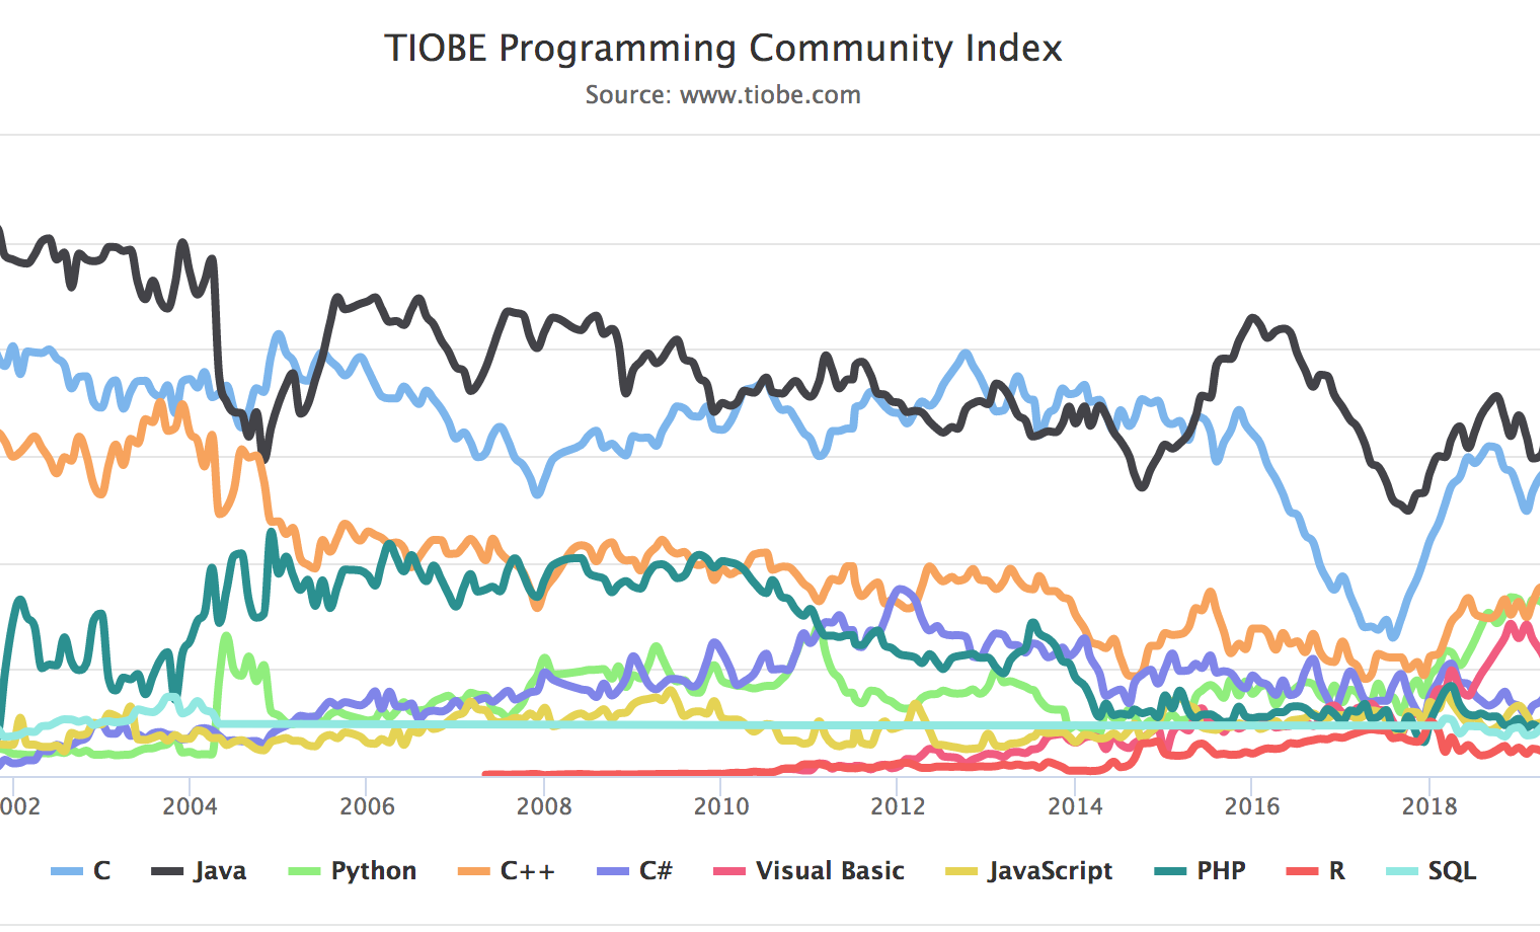
\includegraphics[width=0.95\textwidth]{assets/images/tiobe-index-1.png}
%         \caption{Indice di popolarità del \cplusplus}
%     \end{figure}
% \end{frame}

% \begin{frame}{Popolarità del \cplusplus}
%     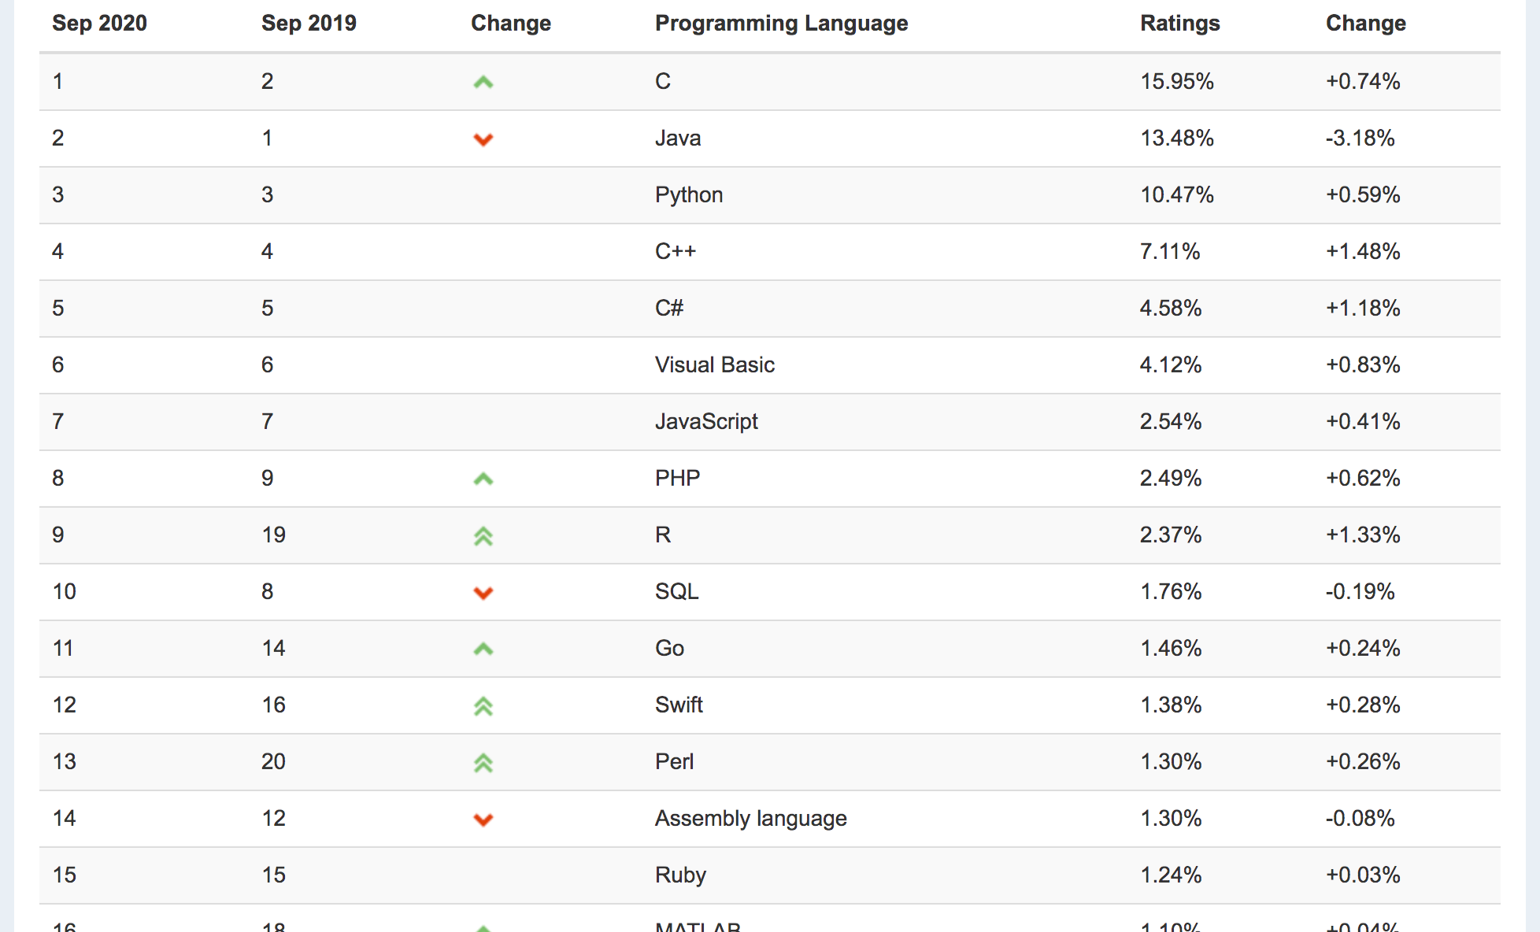
\includegraphics[width=0.95\textwidth]{assets/images/tiobe-index-2.png}
% \end{frame}

% \subsection{\cplusplus evoluzione}

\begin{frame}{Frame Title}
    \begin{itemize}[<+- | alert@+>]
        \item Comunità di utilizzatori
        \item Attori di peso (Microsoft, Google\dots)
        \item Standardizzazione
        \item Opinione: si evolve come un linguaggio naturale
    \end{itemize}
\end{frame}

\subsection{Applicazioni}

\subsection{Principi di progetto del \cplusplus}

\section{Copia profonda in \cplusplus}

\begin{frame}[fragile]{Frame Title}
            \begin{minted}[mathescape,
                tabsize=4,
                fontsize=\scriptsize,
                framesep=2mm]{cpp}
#include <string> // importazione librerie
#include <iostream>

using namespace std; // definizione spazio dei nomi

#ifndef CLASSE_B // guardi di compilazione
#define CLASSE_B

class B {
      string s;
public:
      B(string _s); // costruttore
      string get_s(); // getter
};

#endif
            \end{minted}
\end{frame}

% \subsection{Trucchetti}

% {
%     \metroset{titleformat frame=smallcaps}
% \begin{frame}{Small caps}
% 	This frame uses the \texttt{smallcaps} titleformat.

% 	\begin{alertblock}{Potential Problems}
% 		Be aware, that not every font supports small caps. If for example you typeset your presentation with pdfTeX and the Computer Modern Sans Serif font, every text in smallcaps will be typeset with the Computer Modern Serif font instead.
% 	\end{alertblock}
% \end{frame}
% }

% \section{Elementi}

% \begin{frame}[fragile]{Typography}
%       \begin{verbatim}The theme provides sensible defaults to
% \emph{emphasize} text, \alert{accent} parts
% or show \textbf{bold} results.\end{verbatim}

%   \begin{center}becomes\end{center}

%   The theme provides sensible defaults to \emph{emphasize} text,
%   \alert{accent} parts or show \textbf{bold} results.
% \end{frame}

% \begin{frame}{Font feature test}
%   \begin{itemize}
%     \item Regular
%     \item \textit{Italic}
%     \item \textsc{SmallCaps}
%     \item \textbf{Bold}
%     \item \textbf{\textit{Bold Italic}}
%     \item \textbf{\textsc{Bold SmallCaps}}
%     \item \texttt{Monospace}
%     \item \texttt{\textit{Monospace Italic}}
%     \item \texttt{\textbf{Monospace Bold}}
%     \item \texttt{\textbf{\textit{Monospace Bold Italic}}}
%   \end{itemize}
% \end{frame}

% \begin{frame}{Lists}
%   \begin{columns}[T,onlytextwidth]
%     \column{0.33\textwidth}
%       Items
%       \begin{itemize}
%         \item Milk \item Eggs \item Potatos
%       \end{itemize}

%     \column{0.33\textwidth}
%       Enumerations
%       \begin{enumerate}
%         \item First, \item Second and \item Last.
%       \end{enumerate}

%     \column{0.33\textwidth}
%       Descriptions
%       \begin{description}
%         \item[PowerPoint] Meeh. \item[Beamer] Yeeeha.
%       \end{description}
%   \end{columns}
% \end{frame}

% \begin{frame}{Tables}
%   \begin{table}
%     \caption{Largest cities in the world (source: Wikipedia)}
%     \begin{tabular}{lr}
%       \toprule
%       City & Population\\
%       \midrule
%       Mexico City & 20,116,842\\
%       Shanghai & 19,210,000\\
%       Peking & 15,796,450\\
%       Istanbul & 14,160,467\\
%       \bottomrule
%     \end{tabular}
%   \end{table}
% \end{frame}
% \begin{frame}{Blocks}
%   Three different block environments are pre-defined and may be styled with an
%   optional background color.

%   \begin{columns}[T,onlytextwidth]
%     \column{0.5\textwidth}
%       \begin{block}{Default}
%         Block content.
%       \end{block}

%       \begin{alertblock}{Alert}
%         Block content.
%       \end{alertblock}

%       \begin{exampleblock}{Example}
%         Block content.
%       \end{exampleblock}

%     \column{0.5\textwidth}

%       \metroset{block=fill}

%       \begin{block}{Default}
%         Block content.
%       \end{block}

%       \begin{alertblock}{Alert}
%         Block content.
%       \end{alertblock}

%       \begin{exampleblock}{Example}
%         Block content.
%       \end{exampleblock}

%   \end{columns}
% \end{frame}

% \begin{frame}{Quotes}
%   \begin{quote}
%     Veni, Vidi, Vici
%   \end{quote}
% \end{frame}

% {%
% \setbeamertemplate{frame footer}{My custom footer}
% \begin{frame}[fragile]{Frame footer}
%     \themename defines a custom beamer template to add a text to the footer. It can be set via
%     \begin{verbatim}\setbeamertemplate{frame footer}{My custom footer}\end{verbatim}
% \end{frame}
% }

% \begin{frame}{Riferimenti}
%   Some references to showcase [allowframebreaks] \cite{knuth92,ConcreteMath,Simpson,Er01,greenwade93}
% \end{frame}

% \section{Conclusioni}

% \begin{frame}{Sommario}

%   Get the source of this theme and the demo presentation from

%   \begin{center}\url{github.com/matze/mtheme}\end{center}

%   The theme \emph{itself} is licensed under a
%   \href{http://creativecommons.org/licenses/by-sa/4.0/}{Creative Commons
%   Attribution-ShareAlike 4.0 International License}.

%   \begin{center}\ccbysa\end{center}

% \end{frame}

% {\setbeamercolor{palette primary}{fg=black, bg=yellow}
% \begin{frame}[standout]
%   Questions?
% \end{frame}
% }

% \appendix

% \begin{frame}[fragile]{Backup slides}
%   Sometimes, it is useful to add slides at the end of your presentation to
%   refer to during audience questions.

%   The best way to do this is to include the \verb|appendixnumberbeamer|
%   package in your preamble and call \verb|\appendix| before your backup slides.

%   \themename will automatically turn off slide numbering and progress bars for
%   slides in the appendix.
% \end{frame}

% \begin{frame}[allowframebreaks]{Riferimenti}

%   \bibliography{bibliography}
%   \bibliographystyle{abbrv}

% \end{frame}

\end{document}
